\begin{frame}{Rectified Stereo: Depth from Disparity}
  \begin{columns}[T,onlytextwidth]
    \column{0.48\textwidth}
      \begin{itemize}\footnotesize\itemsep0.3em
        \item \textbf{Rectified rig:} two cameras with the same $K$ (zero skew, $f_x=f_y$, written $f$ and in pixels from here on) and parallel optical axes, centres $C_L$ and $C_R$ a baseline $B$ apart along $x$. A point $\mathbf{X}=(X,Y,Z)^\top$ in left-camera coordinates lands on the same row $v$ in both images.
        \item \textbf{Columns}, by the pinhole model:
        \[ u_L = \frac{fX}{Z}+c_x, \qquad u_R = \frac{f\,(X-B)}{Z}+c_x . \]
        \item \textbf{Disparity} $d = u_L - u_R$ (pixels); $c_x$ cancels:
        \[ d = \frac{fB}{Z} \quad\Longleftrightarrow\quad Z = \frac{fB}{d} \quad (\text{in the units of } B). \]
        \item \textbf{Similar triangles} (shaded; $f$, $d$ as lengths on the image plane): apex $\mathbf{X}$, bases $B$ at depth $0$ and $B-d$ at depth $f$, so $(B-d)/(Z-f) = B/Z$, again $Z = fB/d$. Only $f/d$ enters, so pixel units give the same $Z$.
        \item Depth is inversely proportional to disparity: near points shift a lot, and $d \to 0$ as $Z \to \infty$.
      \end{itemize}
    \column{0.50\textwidth}
      \centering
      \begin{tikzpicture}[font=\sffamily\scriptsize, >=latex]
        % f/Z = 1.4/4 = 0.35, so the points at fraction 0.35 along each ray lie on the image planes
        \coordinate (CL) at (0,0);
        \coordinate (CR) at (3,0);
        \coordinate (X) at (1.2,4);
        \coordinate (xL) at ($(CL)!0.35!(X)$);
        \coordinate (xR) at ($(CR)!0.35!(X)$);
        \fill[blue!8] (CL) -- (CR) -- (X) -- cycle;
        \fill[blue!22] (xL) -- (xR) -- (X) -- cycle;
        \draw[dashed, gray] (CL) -- (0,1.4);
        \draw[dashed, gray] (CR) -- (3,1.4);
        \draw[very thick] (-1.0,1.4) -- (1.0,1.4);
        \draw[very thick] (2.0,1.4) -- (4.0,1.4);
        \draw[thick, red!70!black] (CL) -- (X) -- (CR);
        \fill (CL) circle (1.6pt) node[below=2pt] {$C_L$};
        \fill (CR) circle (1.6pt) node[below=2pt] {$C_R$};
        \fill[red!70!black] (X) circle (1.8pt) node[above=1pt] {$\mathbf{X}$};
        \fill (xL) circle (1.3pt);
        \fill (xR) circle (1.3pt);
        \node at (1.5,1.2) {$B-d$};
        \draw[<->] (0,1.62) -- node[above] {$u_L$} (0.42,1.62);
        \draw[<->] (3,1.62) -- node[above] {$u_R$} (2.37,1.62);
        \draw[gray] (0,-0.45) -- (0,-0.8);
        \draw[gray] (3,-0.45) -- (3,-0.8);
        \draw[<->] (0,-0.68) -- node[below] {$B$} (3,-0.68);
        \draw[gray] (-0.12,0) -- (-1.45,0);
        \draw[gray] (-1.05,1.4) -- (-1.45,1.4);
        \draw[<->] (-1.35,0) -- node[left] {$f$} (-1.35,1.4);
        \draw[gray] (3.12,0) -- (4.65,0);
        \draw[gray, dotted] (1.35,4) -- (4.65,4);
        \draw[<->] (4.55,0) -- node[right] {$Z$} (4.55,4);
        \node[align=left, anchor=west] at (-1.45,2.75) {image planes\\ at depth $f$};
        \draw[gray, ->] (-0.75,2.45) -- (-0.6,1.48);
      \end{tikzpicture}\\[0.2em]
      {\scriptsize Top view. The rays from $C_L$ and $C_R$ meet at $\mathbf{X}$. $u_L$ and $u_R$ are measured from each principal point ($u_R<0$ here).\par}
  \end{columns}
\end{frame}

\begin{frame}{Stereo Rectification}
  \centering
  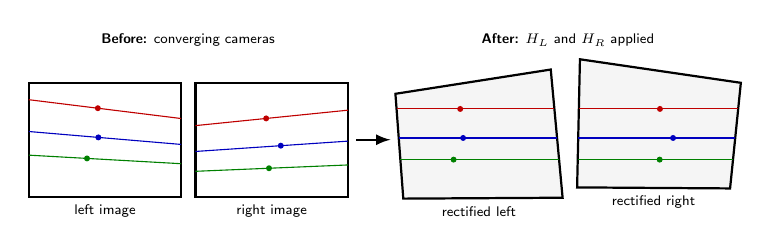
\begin{tikzpicture}[font=\sffamily\scriptsize, >=latex, scale=0.72, every node/.style={transform shape}]
    % Computed example (Python): converging pair with K = diag(500,500,1) + (320,240), baseline along x,
    % rectified as in Fusiello et al. (2000); 0.0042 cm per pixel, image y axis pointing down.
    \node at (2.81,0.75) {\textbf{Before:} converging cameras};
    \node at (9.51,0.75) {\textbf{After:} $H_L$ and $H_R$ applied};
    \draw[thick] (0,0) rectangle (2.688,-2.016);
    \draw[thick] (2.940,0) rectangle (5.628,-2.016);
    \draw[red!75!black] (0,-0.294) -- (2.688,-0.626);
    \draw[red!75!black] (5.628,-0.479) -- (2.940,-0.751);
    \draw[blue!75!black] (0,-0.855) -- (2.688,-1.083);
    \draw[blue!75!black] (5.628,-1.025) -- (2.940,-1.207);
    \draw[green!50!black] (0,-1.272) -- (2.688,-1.423);
    \draw[green!50!black] (5.628,-1.445) -- (2.940,-1.557);
    \fill[red!75!black] (1.218,-0.444) circle (1.5pt);
    \fill[red!75!black] (4.187,-0.624) circle (1.5pt);
    \fill[blue!75!black] (1.227,-0.959) circle (1.5pt);
    \fill[blue!75!black] (4.445,-1.105) circle (1.5pt);
    \fill[green!50!black] (1.027,-1.330) circle (1.5pt);
    \fill[green!50!black] (4.237,-1.503) circle (1.5pt);
    \node at (1.344,-2.25) {left image};
    \node at (4.284,-2.25) {right image};
    \draw[->, thick] (5.78,-1.0) -- (6.38,-1.0);
    \draw[thick, fill=gray!8] (6.467,-0.190) -- (9.207,0.238) -- (9.416,-2.023) -- (6.606,-2.039) -- cycle;
    \draw[thick, fill=gray!8] (9.722,0.419) -- (12.560,0.004) -- (12.370,-1.859) -- (9.672,-1.841) -- cycle;
    \draw[red!75!black] (6.487,-0.457) -- (9.271,-0.457);
    \draw[red!75!black] (9.703,-0.457) -- (12.513,-0.457);
    \draw[blue!75!black] (6.525,-0.969) -- (9.318,-0.969);
    \draw[blue!75!black] (9.691,-0.969) -- (12.461,-0.969);
    \draw[green!50!black] (6.554,-1.351) -- (9.354,-1.351);
    \draw[green!50!black] (9.683,-1.351) -- (12.422,-1.351);
    \fill[red!75!black] (7.610,-0.457) circle (1.5pt);
    \fill[red!75!black] (11.133,-0.457) circle (1.5pt);
    \fill[blue!75!black] (7.661,-0.969) circle (1.5pt);
    \fill[blue!75!black] (11.364,-0.969) circle (1.5pt);
    \fill[green!50!black] (7.493,-1.351) circle (1.5pt);
    \fill[green!50!black] (11.128,-1.351) circle (1.5pt);
    \node at (7.94,-2.27) {rectified left};
    \node at (11.02,-2.1) {rectified right};
  \end{tikzpicture}\\[0.2em]
  {\scriptsize Computed example: three matches and their epipolar lines; after warping, each pair of lines is one row.\par}
  \begin{itemize}\scriptsize\itemsep0.15em
    \item \textbf{Goal:} warp both images by homographies $H_L$, $H_R$ that send both epipoles to infinity along $x$. Matching then becomes a 1D scan along one row.
    \item \textbf{Calibrated method} (after Fusiello et al.\ 2000, who take $\mathbf{r}_1$ along $C_L-C_R$; the sign here keeps the images upright): keep both centres and rotate both cameras to one orientation $R_n=[\mathbf{r}_1\ \mathbf{r}_2\ \mathbf{r}_3]^\top$, whose rows are the new camera axes in world coordinates: $\mathbf{r}_1 = (C_R-C_L)/\lVert C_R-C_L\rVert$ (the baseline), $\mathbf{r}_2 = \mathbf{k}\times\mathbf{r}_1/\lVert\mathbf{k}\times\mathbf{r}_1\rVert$, $\mathbf{r}_3 = \mathbf{r}_1\times\mathbf{r}_2$, where $\mathbf{k}$ is the old left optical axis; give both cameras one $K_n$. Image $i$ is resampled with $H_i = K_n R_n R_i^\top K_i^{-1}$ ($K_i$, $R_i$: original camera) by bilinear interpolation (a distance-weighted blend of the four input pixels around each source position).
    \item \textbf{Limits:} the construction fails for forward motion along the optical axis, where the epipole lies inside the image. Loop and Zhang (1999) need only the epipolar geometry ($F$) and choose $H_L$, $H_R$ to minimise image distortion.
  \end{itemize}
  \vspace{0.1em}
  {\scriptsize Fusiello, Trucco, and Verri, ``A Compact Algorithm for Rectification of Stereo Pairs,'' \textit{Machine Vision and Applications} 12(1), 2000, \href{https://doi.org/10.1007/s001380050120}{doi:10.1007/s001380050120}, Sections~3--4; Loop and Zhang, ``Computing Rectifying Homographies for Stereo Vision,'' CVPR 1999, \href{https://doi.org/10.1109/CVPR.1999.786928}{doi:10.1109/CVPR.1999.786928}.\par}
\end{frame}

\begin{frame}{Depth Resolution Falls with Distance}
  \begin{itemize}\footnotesize\itemsep0.25em
    \item Differentiating $Z = fB/d$: a matching error of $\Delta d$ pixels gives
    \[ \Delta Z \approx \Big|\frac{\partial Z}{\partial d}\Big|\,\Delta d = \frac{Z^2}{fB}\,\Delta d, \qquad \frac{\Delta Z}{Z} \approx \frac{Z}{fB}\,\Delta d . \]
    \item \textbf{KITTI} (car-mounted rig, 2011-09-26 calibration, grayscale pair): rectified $f = 721.54$\,px and $fB = 387.57$ pixel-metres, so $B = 0.537$\,m; the paper gives both stereo baselines as approximately 54\,cm.
  \end{itemize}
  \vspace{0.1em}
  {\centering\scriptsize
  \begin{tabular}{r r r r r}
    \toprule
    \textbf{Depth $Z$} & \textbf{Disparity $d = fB/Z$} & \textbf{$\Delta Z$ at $\Delta d = 1$\,px} & \textbf{$\Delta Z/Z$} & \textbf{$Z$ at $d \pm 1$\,px} \\
    \midrule
    5\,m & 77.5\,px & 0.06\,m & 1.3\% & 4.94--5.07\,m \\
    10\,m & 38.8\,px & 0.26\,m & 2.6\% & 9.75--10.26\,m \\
    20\,m & 19.4\,px & 1.03\,m & 5.2\% & 19.02--21.09\,m \\
    50\,m & 7.8\,px & 6.45\,m & 12.9\% & 44.29--57.41\,m \\
    \bottomrule
  \end{tabular}\par}
  \vspace{0.2em}
  \begin{itemize}\footnotesize\itemsep0.25em
    \item \textbf{Levers:} a longer baseline or a longer focal length divides every $\Delta Z$ by the same factor; sub-pixel matching shrinks $\Delta d$ itself (at $0.25$\,px every $\Delta Z$ above drops fourfold).
    \item \textbf{Trade-offs:} doubling $B$ also doubles every disparity. With a search range of $D = 192$ disparities ($d \leq 191$), the nearest measurable depth $fB/(D-1)$ moves from $2.0$\,m to $4.1$\,m, and the region both cameras see starts farther out. A longer $f$ narrows the field of view.
  \end{itemize}
  \vspace{0.1em}
  {\scriptsize Geiger et al., ``Vision Meets Robotics: The KITTI Dataset,'' \textit{IJRR} 32(11), 2013, \href{https://doi.org/10.1177/0278364913491297}{doi:10.1177/0278364913491297}, Section~II; raw-data calibration \texttt{2011\_09\_26/calib\_cam\_to\_cam.txt}, cameras 0 and 1.\par}
\end{frame}

\begin{frame}{Matching Costs and the Cost Volume}
  \begin{columns}[T,onlytextwidth]
    \column{0.58\textwidth}
      \begin{itemize}\scriptsize\itemsep0.12em
        \item \textbf{Matching cost} $C(\mathbf{p},d)$: left pixel $\mathbf{p}=(u,v)$ against right pixel $(u-d,v)$ over a window $\mathcal{W}$, e.g.\ the sum of absolute differences (SAD)
        \[ C_{\mathrm{SAD}}(\mathbf{p},d) = \textstyle\sum_{(i,j)\in \mathcal{W}} \big|I_L(u{+}i,v{+}j) - I_R(u{+}i{-}d,v{+}j)\big| . \]
        Squared differences (SSD) work alike; normalized cross-correlation (NCC) of zero-mean, unit-norm windows cancels gain and bias.
        \item \textbf{Census transform:} one bit per neighbour, 1 when it is darker than the centre; the cost is the Hamming distance between the two bit strings. Only comparisons count: gain and bias cancel, and an outlier neighbour flips only its own bit.
        \item \textbf{Cost volume} $C(u,v,d)$, $d \in \{0,\dots,D-1\}$: an $H\times W\times D$ array (the disparity space image of Scharstein and Szeliski). Winner-take-all: $d_{\mathbf{p}} = \operatorname*{arg\,min}_d C(\mathbf{p},d)$.
        \item \textbf{Failures:} textureless regions (flat cost curve), repetitive patterns (several minima), occlusions (no true match), specular surfaces (view-dependent appearance).
        \item \textbf{Left-right check:} with disparity maps $d_L$ and $d_R$ of both images, keep $\mathbf{p}$ only if $|d_L(u,v) - d_R(u - d_L(u,v), v)| \leq 1$.
      \end{itemize}
    \column{0.40\textwidth}
      \centering
      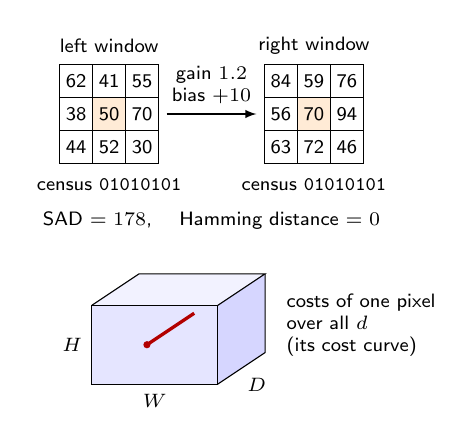
\begin{tikzpicture}[font=\sffamily\scriptsize, >=latex,
          cell/.style={draw, minimum size=0.42cm, inner sep=0pt},
          ctr/.style={cell, fill=orange!16}]
        \node at (0.42,0.45) {left window};
        \node[cell] at (0,0) {62}; \node[cell] at (0.42,0) {41}; \node[cell] at (0.84,0) {55};
        \node[cell] at (0,-0.42) {38}; \node[ctr] at (0.42,-0.42) {50}; \node[cell] at (0.84,-0.42) {70};
        \node[cell] at (0,-0.84) {44}; \node[cell] at (0.42,-0.84) {52}; \node[cell] at (0.84,-0.84) {30};
        \node at (3.02,0.45) {right window};
        \node[cell] at (2.6,0) {84}; \node[cell] at (3.02,0) {59}; \node[cell] at (3.44,0) {76};
        \node[cell] at (2.6,-0.42) {56}; \node[ctr] at (3.02,-0.42) {70}; \node[cell] at (3.44,-0.42) {94};
        \node[cell] at (2.6,-0.84) {63}; \node[cell] at (3.02,-0.84) {72}; \node[cell] at (3.44,-0.84) {46};
        \draw[->] (1.15,-0.42) -- node[above, align=center] {gain $1.2$\\ bias $+10$} (2.29,-0.42);
        \node at (0.42,-1.32) {census \texttt{01010101}};
        \node at (3.02,-1.32) {census \texttt{01010101}};
        \node at (1.72,-1.78) {SAD $= 178$, \quad Hamming distance $= 0$};
        % cost volume: front face W x H, the disparity axis drawn obliquely
        \begin{scope}[shift={(0.2,-3.85)}]
          \fill[blue!10] (0,0) rectangle (1.6,1.0);
          \fill[blue!5] (0,1.0) -- (0.6,1.4) -- (2.2,1.4) -- (1.6,1.0) -- cycle;
          \fill[blue!16] (1.6,0) -- (2.2,0.4) -- (2.2,1.4) -- (1.6,1.0) -- cycle;
          \draw (0,0) rectangle (1.6,1.0);
          \draw (0,1.0) -- (0.6,1.4) -- (2.2,1.4) -- (1.6,1.0);
          \draw (1.6,0) -- (2.2,0.4) -- (2.2,1.4);
          \draw[very thick, red!70!black] (0.7,0.5) -- (1.3,0.9);
          \fill[red!70!black] (0.7,0.5) circle (1.3pt);
          \node[below] at (0.8,0) {$W$};
          \node[left] at (0,0.5) {$H$};
          \node[below right] at (1.85,0.2) {$D$};
          \node[anchor=west, align=left] at (2.35,0.75) {costs of one pixel\\ over all $d$\\ (its cost curve)};
        \end{scope}
      \end{tikzpicture}\\[0.2em]
      {\scriptsize Census bits in raster order, centre skipped.\par}
  \end{columns}
  \vspace{0.1em}
  {\scriptsize Zabih and Woodfill, ``Non-parametric Local Transforms for Computing Visual Correspondence,'' ECCV 1994, \href{https://doi.org/10.1007/BFb0028345}{doi:10.1007/BFb0028345}, Section~3; Scharstein and Szeliski, ``A Taxonomy and Evaluation of Dense Two-Frame Stereo Correspondence Algorithms,'' \textit{IJCV} 47(1--3), 2002, \href{https://doi.org/10.1023/A:1014573219977}{doi:10.1023/A:1014573219977}; left-right check: Hirschm\"uller (next slide), Eq.~15.\par}
\end{frame}

\begin{frame}{Semi-Global Matching}
  \begin{columns}[T,onlytextwidth]
    \column{0.62\textwidth}
      \begin{itemize}\scriptsize\itemsep0.12em
        \item \textbf{Energy} of a disparity map, with neighbours $\mathcal{N}_{\mathbf{p}}$ and $[\cdot]$ equal to $1$ when true:
        \[ E(d) = \sum_{\mathbf{p}} C(\mathbf{p},d_{\mathbf{p}}) + \sum_{\mathbf{p}}\sum_{\mathbf{q}\in\mathcal{N}_{\mathbf{p}}} \Big( P_1[|d_{\mathbf{p}}-d_{\mathbf{q}}|=1] + P_2[|d_{\mathbf{p}}-d_{\mathbf{q}}|>1] \Big) \]
        A small $P_1$ allows slanted and curved surfaces; a larger $P_2 \geq P_1$ charges every jump the same, which keeps depth edges sharp.
        \item Minimising $E$ over the 2D image is NP-complete for such energies (no known algorithm solves every instance in time polynomial in the image size). Along a 1D path it is exact by \textbf{dynamic programming}: each pixel reuses the best costs of the previous pixel $\mathbf{p}-\mathbf{r}$ along direction $\mathbf{r}$,
        \[ \begin{aligned} L_{\mathbf{r}}(\mathbf{p},d) &= C(\mathbf{p},d) + \min\big( L_{\mathbf{r}}(\mathbf{p}{-}\mathbf{r},d),\; L_{\mathbf{r}}(\mathbf{p}{-}\mathbf{r},d{-}1){+}P_1,\\ &\qquad L_{\mathbf{r}}(\mathbf{p}{-}\mathbf{r},d{+}1){+}P_1,\; \min\nolimits_i L_{\mathbf{r}}(\mathbf{p}{-}\mathbf{r},i){+}P_2 \big)\\ &\quad - \min\nolimits_k L_{\mathbf{r}}(\mathbf{p}{-}\mathbf{r},k). \end{aligned} \]
        The last term keeps the values bounded without moving the minimum.
        \item \textbf{Aggregate} $S(\mathbf{p},d) = \sum_{\mathbf{r}} L_{\mathbf{r}}(\mathbf{p},d)$ over at least 8 paths, 16 recommended, then winner-take-all on $S$. Cost $O(WHD)$.
      \end{itemize}
    \column{0.36\textwidth}
      \centering
      \begin{tikzpicture}[font=\sffamily\scriptsize, >=latex, scale=0.68]
        \draw[gray!35, step=0.3] (-1.05,-1.05) grid (1.05,1.05);
        \fill[orange!45] (-0.15,-0.15) rectangle (0.15,0.15);
        \node at (0,0) {$\mathbf{p}$};
        \foreach \a in {0,45,...,315}
          \draw[-{Latex[length=1.3mm]}, thick, blue!70!black] (\a:1.55) -- (\a:0.55);
        \foreach \a in {26.57,63.43,116.57,153.43,206.57,243.43,296.57,333.43}
          \draw[-{Latex[length=1.3mm]}, densely dashed, red!70!black] (\a:1.55) -- (\a:0.55);
      \end{tikzpicture}\\[0.2em]
      {\scriptsize Paths into $\mathbf{p}$: 8 solid, plus 8 dashed for 16.\par}
      \vspace{0.2em}
      \begin{itemize}\scriptsize\itemsep0.1em
        \item \textbf{Speed:} 1--2\,s on typical test images (Teddy, $450{\times}375$: 1.8\,s on a 2.2\,GHz CPU).
        \item \textbf{Deployed:} Daimler ran it on a low-power field-programmable gate array (FPGA) for driver assistance (27\,Hz, under 3\,W); by 2011 the German Aerospace Center (DLR) had run it on over 100\,TB of aerial and satellite images.
        \item OpenCV ships a variant, \texttt{StereoSGBM}: 5 directions by default, 8 in full mode (\href{https://docs.opencv.org/4.x/d2/d85/classcv_1_1StereoSGBM.html}{docs.opencv.org}).
      \end{itemize}
  \end{columns}
  \vspace{0.1em}
  {\scriptsize Hirschm\"uller, ``Stereo Processing by Semiglobal Matching and Mutual Information,'' \textit{IEEE TPAMI} 30(2), 2008, \href{https://doi.org/10.1109/TPAMI.2007.1166}{doi:10.1109/TPAMI.2007.1166}, Eqs.~11--15; Hirschm\"uller, ``Semi-Global Matching: Motivation, Developments and Applications,'' Photogrammetric Week 2011, pp.~173--184.\par}
\end{frame}

\begin{frame}{Learned Stereo: Cost Volumes and Soft Argmin}
  \centering
  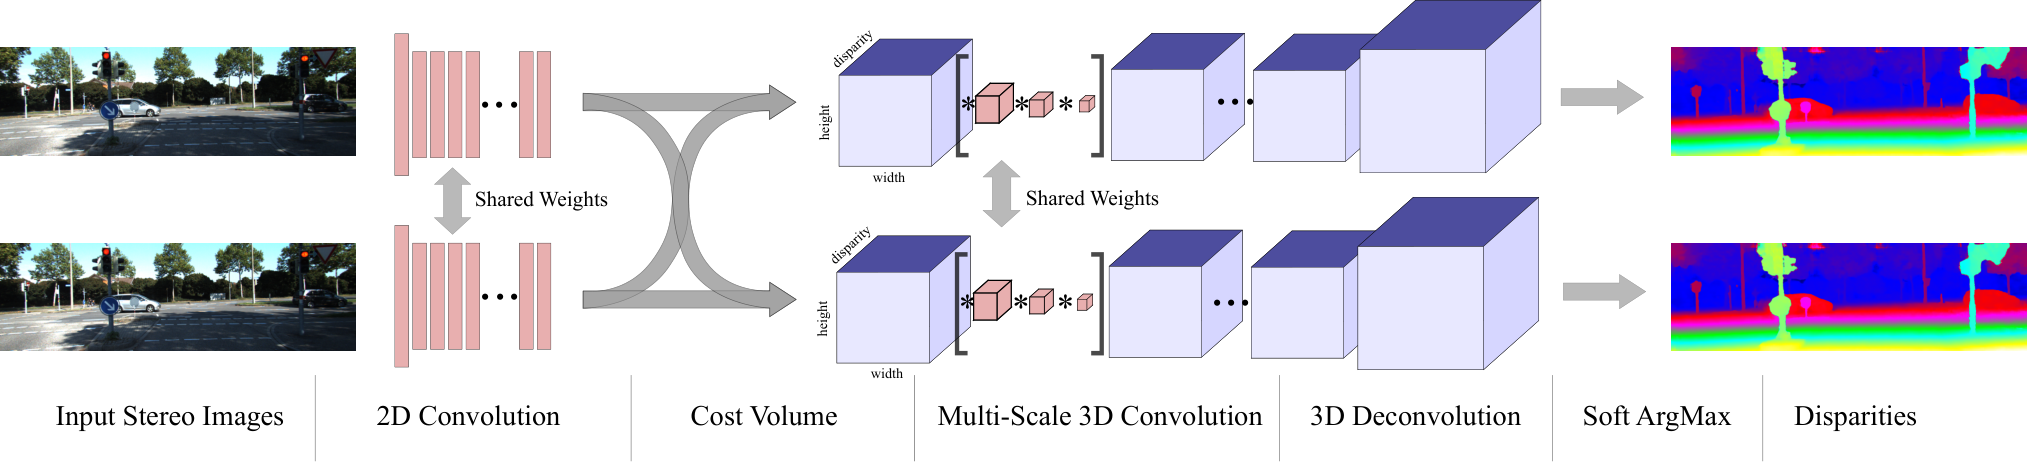
\includegraphics[width=\textwidth,height=0.26\textheight,keepaspectratio]{images/3d-vision/gcnet_fig1_architecture.png}\\[0.2em]
  {\scriptsize Kendall et al., ``End-to-End Learning of Geometry and Context for Deep Stereo Regression,'' ICCV 2017, \href{https://arxiv.org/abs/1703.04309v1}{arXiv:1703.04309v1}, Figure~1.\par}
  \begin{columns}[T,onlytextwidth]
    \column{0.49\textwidth}
      \begin{itemize}\scriptsize\itemsep0.2em
        \item \textbf{GC-Net:} one 2D CNN with shared weights computes features for both images. For each disparity level, the left feature at $(u,v)$ is concatenated with the right feature at $(u-d,v)$: a 4D cost volume (height, width, disparity, feature).
        \item \textbf{3D convolutions} in an encoder-decoder turn it into one cost $c_d$ per pixel and disparity.
        \item \textbf{Soft argmin} (``Soft ArgMax'' in the figure): $\hat d = \sum_{d=0}^{D-1} d\cdot\sigma_d(-\mathbf{c})$, with $\sigma$ the softmax over the $D$ costs $\mathbf{c}$ of a pixel. It is differentiable and gives sub-pixel disparities; training minimises the L1 error $|d-\hat d|$ on pixels with ground truth.
      \end{itemize}
    \column{0.49\textwidth}
      \begin{itemize}\scriptsize\itemsep0.2em
        \item \textbf{PSMNet:} spatial pyramid pooling averages the features over $64{\times}64$, $32{\times}32$, $16{\times}16$ and $8{\times}8$ windows, then upsamples and concatenates them, so each pixel carries context at four scales.
        \item \textbf{Stacked hourglass:} three 3D encoder-decoders in a row, each predicting a disparity map with its own loss.
        \item \textbf{Metrics:} end-point error (EPE), the mean $|\hat d - d|$ in pixels; KITTI~2015 \textbf{D1}, the share of pixels whose error is $\geq 3$\,px and $\geq 5\%$ of the true disparity.
        \item GC-Net $\to$ PSMNet: EPE $2.51 \to 1.09$\,px on Scene Flow (rendered scenes); D1 over all pixels $2.87\% \to 2.32\%$ on the KITTI~2015 test set.
      \end{itemize}
  \end{columns}
  \vspace{0.1em}
  {\scriptsize Chang and Chen, ``Pyramid Stereo Matching Network,'' CVPR 2018, \href{https://arxiv.org/abs/1803.08669v1}{arXiv:1803.08669v1}, Sections~3.2--3.4, Tables~4--5; D1: KITTI 2015 stereo benchmark, \href{https://www.cvlibs.net/datasets/kitti/eval_scene_flow.php?benchmark=stereo}{cvlibs.net/datasets/kitti}.\par}
\end{frame}

\begin{frame}{Iterative Refinement: RAFT-Stereo}
  \begin{itemize}\scriptsize\itemsep0.1em
    \item \textbf{RAFT} (optical flow as a dense motion field): a CNN $g$ maps both frames to features at $1/8$ resolution. The \textbf{correlation volume} holds the dot product of every pair of feature vectors, $C_{ijkl} = \sum_h g(I_1)_{ijh}\, g(I_2)_{klh}$, average-pooled into a 4-level pyramid.
    \item \textbf{Recurrent updates:} the flow starts at $0$. Each iteration, a lookup $L_C$ reads the correlations within radius $r$ of the current estimate at every pyramid level, and a convolutional GRU (a GRU with convolutions in place of its fully connected layers) predicts an increment.
    \item \textbf{RAFT-Stereo:} matches share a row, so only same-row pairs are kept, $C_{ijk} = \sum_h g(I_L)_{ijh}\, g(I_R)_{ikh}$ ($H{\times}W{\times}W$), pooled along the last axis only. GRUs at $1/8$, $1/16$ and $1/32$ resolution exchange hidden states, spreading context across textureless regions. No 3D convolutions: megapixel images fit. Loss: L1 on iterate $i$ of $N$, weighted $0.9^{N-i}$.
    \item \textbf{Zero-shot test} (trained on Scene Flow only, no training on any test dataset), \% of pixels above the error threshold. KITTI 2015: driving; Middlebury: indoor, half resolution; ETH3D: indoor and outdoor.
  \end{itemize}
  \vspace{0.1em}
  {\centering\scriptsize
  \begin{tabular}{l c c c}
    \toprule
    & \textbf{KITTI 2015, 3\,px} & \textbf{Middlebury, 2\,px} & \textbf{ETH3D, 1\,px} \\
    \midrule
    PSMNet & 16.3 & 25.1 & 23.8 \\
    RAFT-Stereo & 5.74 & 12.59 & 3.28 \\
    \bottomrule
  \end{tabular}\par}
  \vspace{0.2em}
  {\scriptsize Table~1. Fine-tuned on Middlebury, RAFT-Stereo ranked first there at submission, its 1\,px error 29\% below the next method.\par}
  \vspace{0.2em}
  {\scriptsize Teed and Deng, ``RAFT: Recurrent All-Pairs Field Transforms for Optical Flow,'' ECCV 2020, \href{https://arxiv.org/abs/2003.12039v3}{arXiv:2003.12039v3}; Lipson, Teed, and Deng, ``RAFT-Stereo: Multilevel Recurrent Field Transforms for Stereo Matching,'' 3DV 2021, \href{https://arxiv.org/abs/2109.07547v1}{arXiv:2109.07547v1}.\par}
\end{frame}

\begin{frame}{RAFT-Stereo: Architecture}
  \centering
  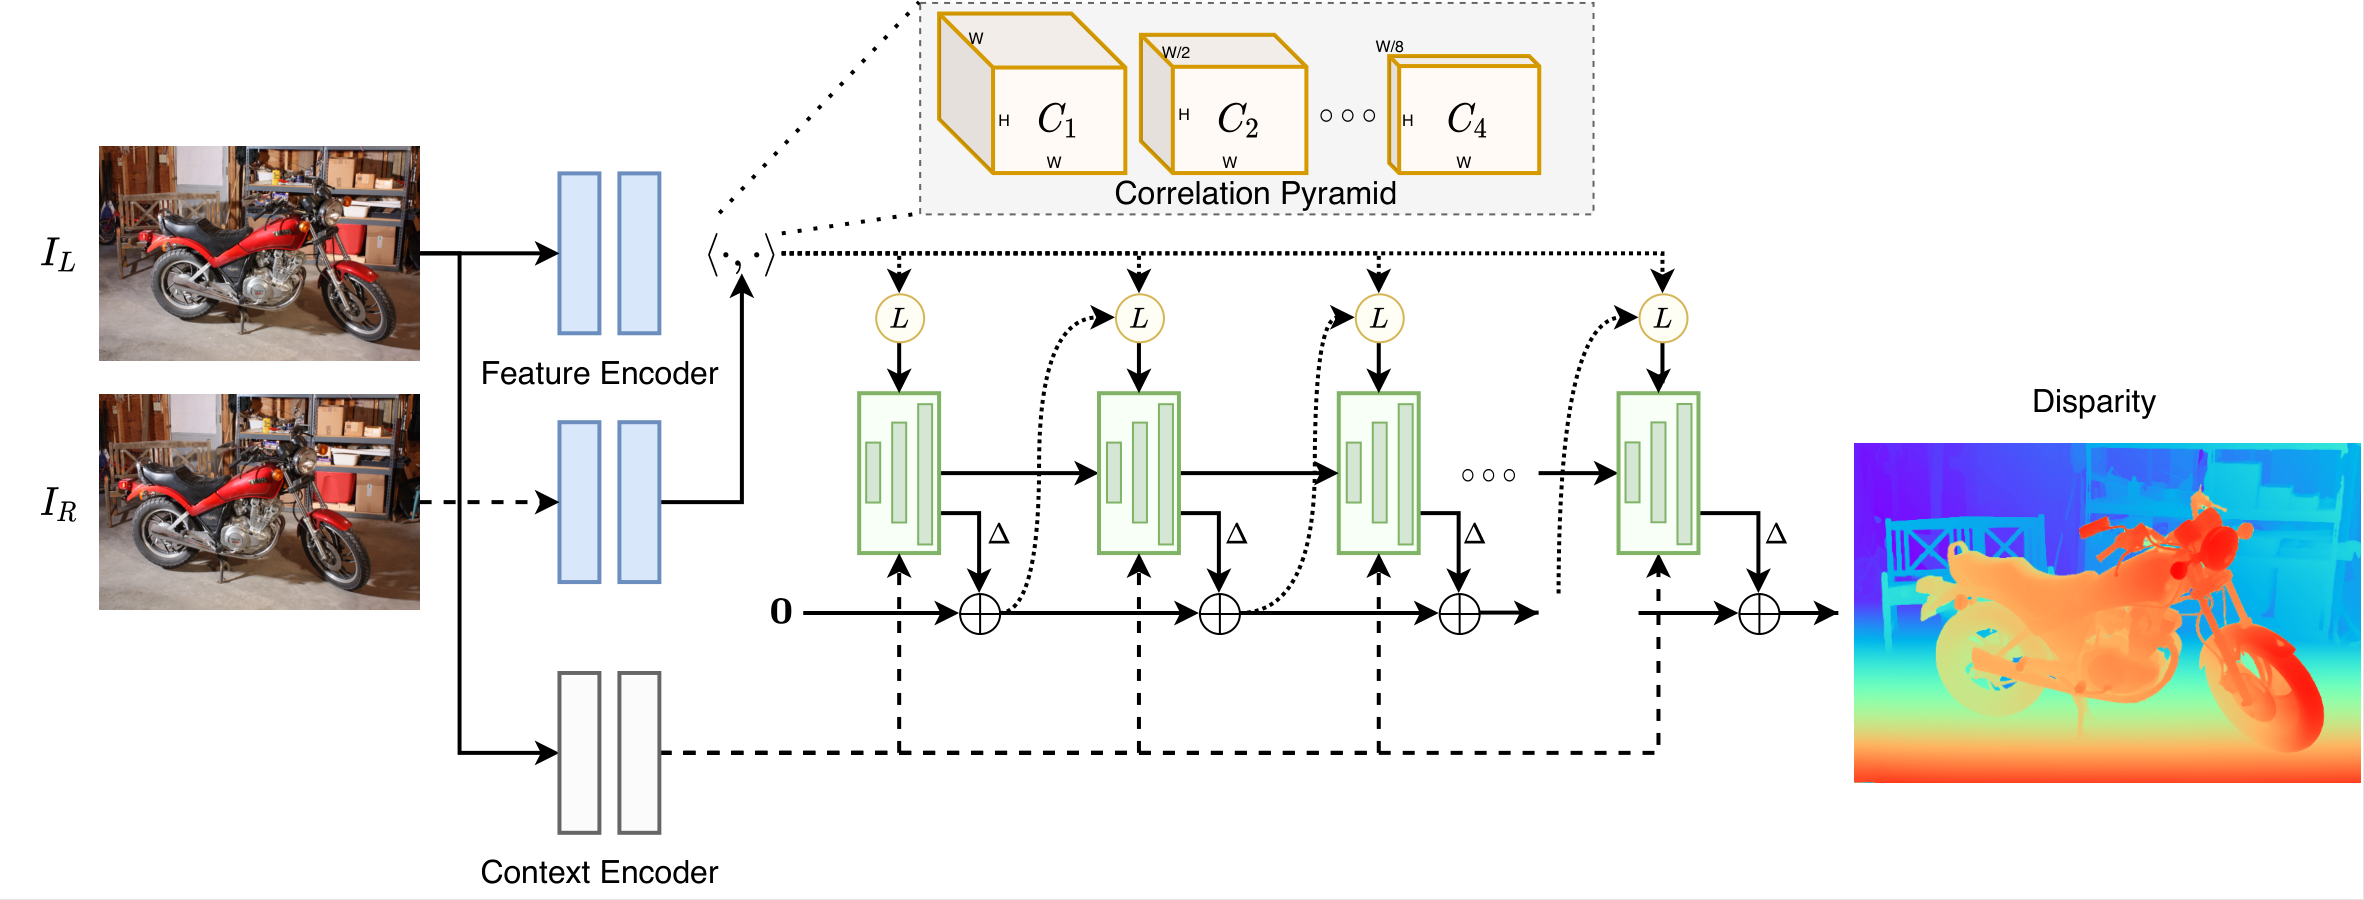
\includegraphics[width=\textwidth,height=0.70\textheight,keepaspectratio]{images/3d-vision/raftstereo_fig1_architecture.png}\\[0.2em]
  {\scriptsize Lipson, Teed, and Deng, \href{https://arxiv.org/abs/2109.07547v1}{arXiv:2109.07547v1}, Figure~1.\par}
  \vspace{0.3em}
  \begin{itemize}\scriptsize\itemsep0.15em
    \item \textbf{Blue:} the feature encoder runs on $I_L$ and $I_R$; same-row dot products $\langle\cdot,\cdot\rangle$ build the correlation pyramid $C_1,\dots,C_4$. \textbf{White:} the context encoder sees $I_L$ only; it sets the GRUs' initial hidden state and feeds every GRU step.
    \item \textbf{Green:} from disparity $\mathbf{0}$, each GRU step looks up the pyramid ($L$) at the current estimate and adds an update $\Delta$; the final estimate is upsampled to full resolution.
  \end{itemize}
\end{frame}

\begin{frame}{Stereo Foundation Models: FoundationStereo}
  \begin{itemize}\scriptsize\itemsep0.25em
    \item \textbf{Goal:} one model that works zero-shot in new domains.
    \item \textbf{Data:} the FoundationStereo dataset (FSD), 1M synthetic stereo pairs; a self-curation loop drops ambiguous pairs (repeated texture, reflections, flat colour) and replaces them with newly generated ones.
    \item \textbf{Side-Tuning Adapter (STA):} features of a frozen Depth Anything~V2 plus a trainable CNN bring monocular priors learned on real images.
    \item \textbf{Attentive Hybrid Cost Filtering (AHCF):} a cost volume of group-wise correlations (feature channels split into 8 groups, one dot product per group) and concatenated features, filtered by axial-planar convolutions (a 3D convolution split into spatial and disparity parts) and a Disparity Transformer (self-attention along disparity).
    \item A soft argmin gives the initial disparity; convolutional GRU updates refine it as in RAFT-Stereo.
  \end{itemize}
  \vspace{0.1em}
  {\centering\scriptsize
  \begin{tabular}{l l c c}
    \toprule
    \textbf{Model} & \textbf{Training data} & \textbf{Middlebury BP-2} & \textbf{ETH3D BP-1} \\
    \midrule
    RAFT-Stereo & Scene Flow & 12.6 & 3.3 \\
    FoundationStereo & Scene Flow & 5.5 & 1.8 \\
    FoundationStereo & FSD + 6 public sets & 1.1 & 0.5 \\
    \bottomrule
  \end{tabular}\par}
  \vspace{0.2em}
  {\scriptsize Zero-shot results (Table~2). BP-$X$: \% of pixels with error above $X$ px; no method saw the target datasets. Fine-tuned, FoundationStereo ranked first on the ETH3D and Middlebury leaderboards at submission.\par}
  \vspace{0.2em}
  {\scriptsize Wen et al., ``FoundationStereo: Zero-Shot Stereo Matching,'' CVPR 2025, \href{https://arxiv.org/abs/2501.09898v4}{arXiv:2501.09898v4}, Sections~3--4.\par}
\end{frame}

\begin{frame}{FoundationStereo: Architecture}
  \centering
  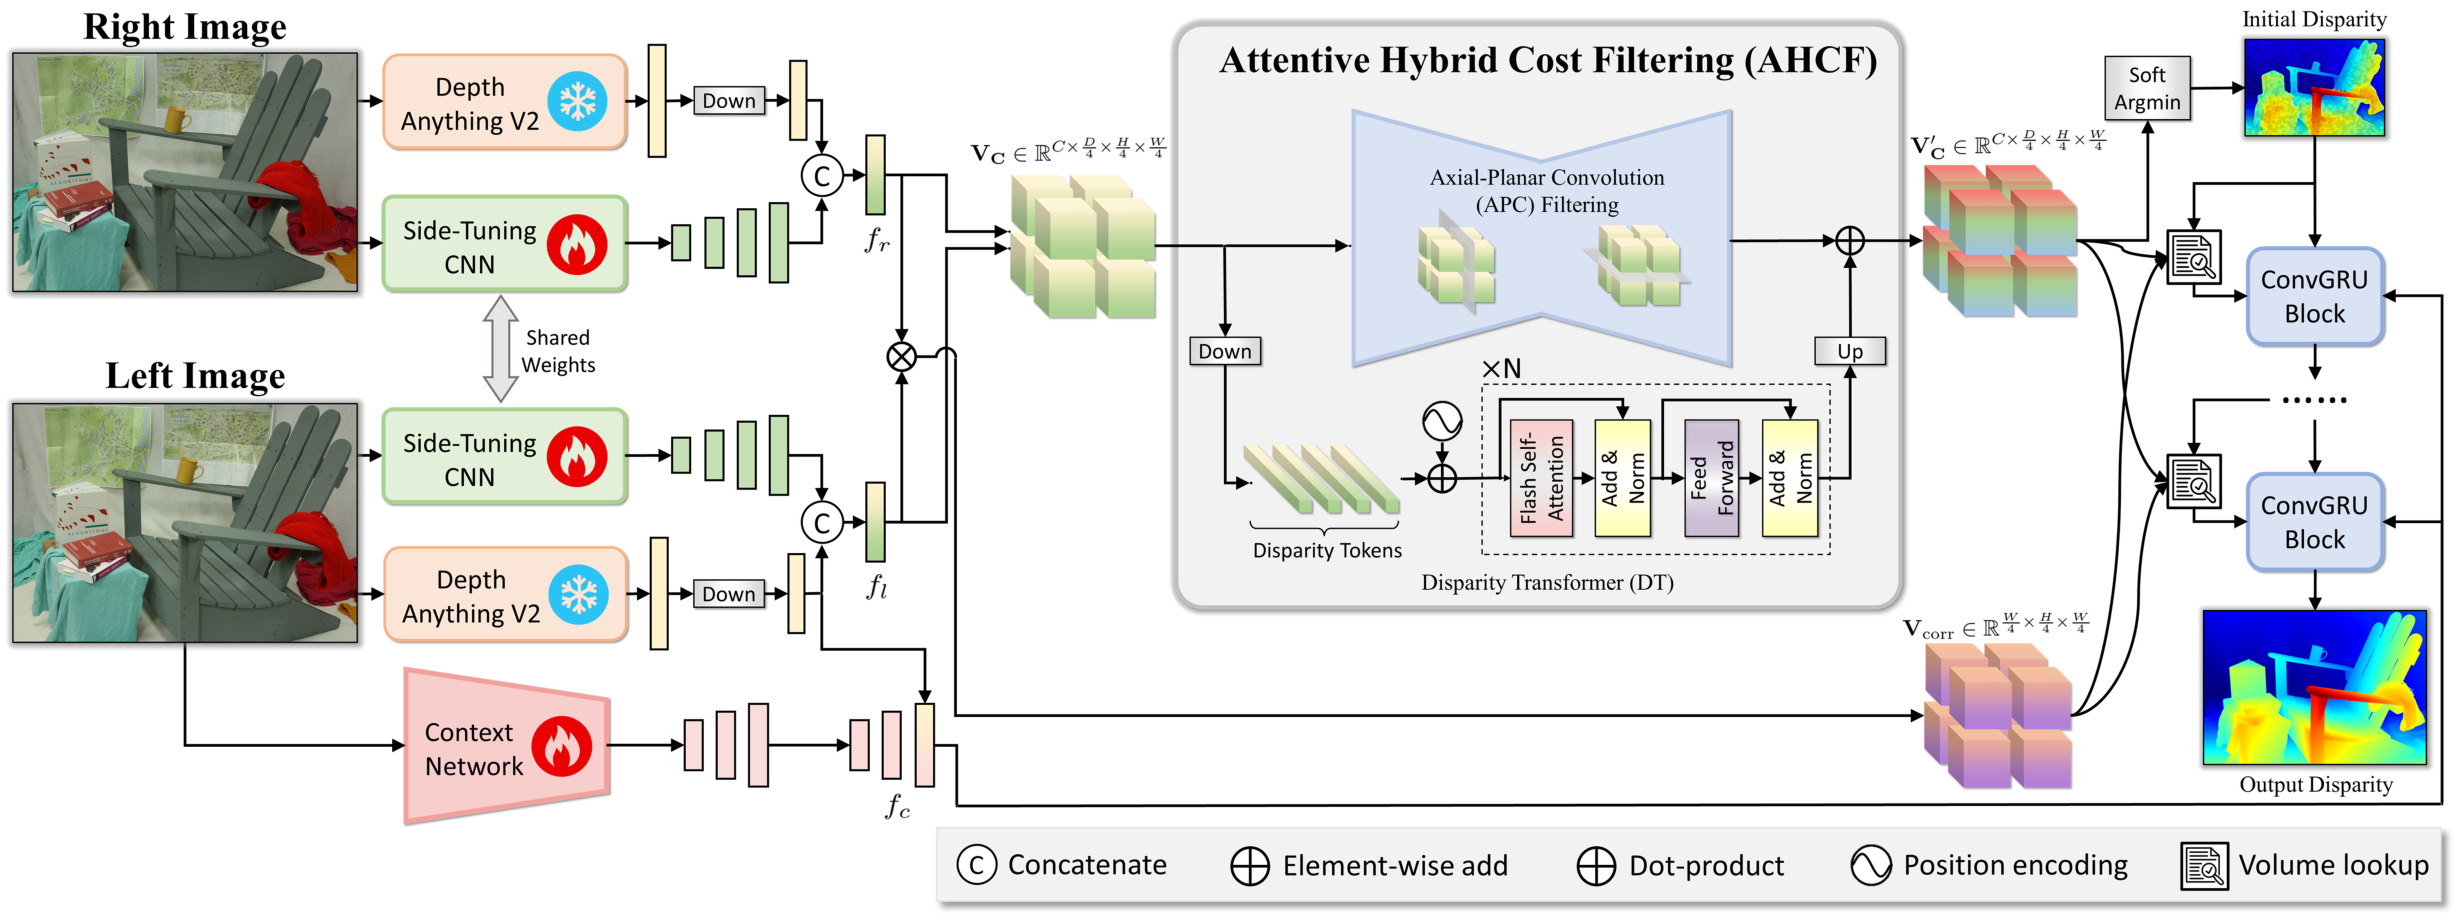
\includegraphics[width=\textwidth,height=0.70\textheight,keepaspectratio]{images/3d-vision/foundationstereo_fig2_overview.png}\\[0.2em]
  {\scriptsize Wen et al., \href{https://arxiv.org/abs/2501.09898v4}{arXiv:2501.09898v4}, Figure~2.\par}
  \vspace{0.3em}
  \begin{itemize}\scriptsize\itemsep0.15em
    \item \textbf{Left:} frozen Depth Anything~V2 (snowflake) plus trainable side-tuning CNN (flame) give $f_l$, $f_r$; the context network sees the left image only. \textbf{Middle:} AHCF filters the hybrid volume $\mathbf{V_C}$ (APC, DT); a soft argmin gives the initial disparity.
    \item \textbf{Right:} convolutional GRU blocks refine it, looking up the filtered volume and the correlation volume $\mathbf{V}_{\mathrm{corr}}$.
  \end{itemize}
\end{frame}

\begin{frame}{Active Depth Sensing}
  \begin{itemize}\scriptsize\itemsep0.1em
    \item \textbf{Structured light:} a projector replaces the second camera. The shift of its known pattern in the camera image is a disparity, so $Z = fb/d$ as in stereo, with projector-camera baseline $b$.
    \item \textbf{Time of flight (ToF):} light goes to the surface and back, so the distance along the pixel's ray is $\ell = ct/2$ ($c$: speed of light, $t$: round-trip time), and the depth is $Z = \ell/\lVert K^{-1}\tilde{\mathbf{x}}\rVert \leq \ell$. ToF cameras read $t$ from the phase $\varphi = 2\pi f_m t$ of light modulated at $f_m$, which wraps beyond $\ell = c/(2f_m)$; several frequencies are combined. \textbf{LiDAR} (light detection and ranging) times laser pulses along scanned beams.
  \end{itemize}
  \vspace{0.1em}
  {\centering\scriptsize\setlength{\tabcolsep}{4pt}
  \begin{tabular}{>{\raggedright\arraybackslash}p{2.6cm} >{\raggedright\arraybackslash}p{2.7cm} >{\raggedright\arraybackslash}p{2.3cm} >{\raggedright\arraybackslash}p{5.2cm}}
    \toprule
    \textbf{Sensor (example)} & \textbf{Output} & \textbf{Range, accuracy} & \textbf{Weaknesses} \\
    \midrule
    Structured light (first Kinect) & $640{\times}480$ depth, 30\,Hz & short: $b = 7.5$\,cm & sunlight swamps the pattern; devices interfere \\
    \addlinespace[0.1em]
    ToF camera (Kinect One) & $512{\times}424$ depth & driver cuts off near 4.5\,m & multipath (light arriving via other surfaces); mixed pixels at depth edges; interference \\
    \addlinespace[0.1em]
    LiDAR (Velodyne HDL-64E, KITTI) & 64 beams, 10\,Hz; about 120K points per scan & 120\,m, 2\,cm accuracy & sparse; fog, rain, snow; sunlight and other LiDARs interfere; cost, moving parts \\
    \addlinespace[0.1em]
    Passive stereo (KITTI rig) & every pixel, $1242{\times}375$ & error grows as $Z^2/(fB)$ & textureless and repetitive regions, occlusions, darkness \\
    \bottomrule
  \end{tabular}\par}
  \vspace{0.1em}
  \begin{itemize}\scriptsize\itemsep0.1em
    \item \textbf{Passive stereo wins} on cost, resolution and outdoor use: cameras emit nothing, so sunlight and other vehicles do not interfere, and range scales with $B$ and $f$. Active sensors win on blank walls, in the dark, and (LiDAR) at long range.
  \end{itemize}
  {\scriptsize Sarbolandi, Lefloch, and Kolb, ``Kinect Range Sensing: Structured-Light versus Time-of-Flight Kinect,'' \textit{CVIU} 139, 2015, \href{https://arxiv.org/abs/1505.05459v1}{arXiv:1505.05459v1}, Sections~1--2, Table~2; Li and Ibanez-Guzman, ``Lidar for Autonomous Driving: The Principles, Challenges, and Trends for Automotive Lidar and Perception Systems,'' \textit{IEEE Signal Processing Magazine} 37(4), 2020, \href{https://arxiv.org/abs/2004.08467v1}{arXiv:2004.08467v1}, Eq.~2; HDL-64E: Geiger et al.\ 2013, Sections~II and~III-A.\par}
\end{frame}
